% vi:ft=tex

\section{Problem statement}

\paragraph{}
\glssymbol{pbs} is a workload management system which optimizes \gls{job}
scheduling in \gls{hpc} environments --- clusters, clouds and super computers.
\gls{spark} is a data analytics engine for large-scale data processing and has a
standalone cluster manager which handles the spark jobs sent to a cluster of
nodes. But for both of these, their own daemons should be running on the nodes
and should have information about the node like number of CPU cores, memory
available for use etc. Since they are two completely different programs, they
have no way of knowing which node is in use by the other program at a given time
and thus create problems when scheduling.

\paragraph{}
The current workaround for the said problem is to segregate the nodes cluster
into two partitions --- \glssymbol{hpc} cluster and \gls{spark} cluster. But
this creates another problem. At any given time if the demand for running
\glssymbol{hpc} jobs is high and the demand for \gls{spark} jobs is low, the
\gls{spark} cluster will remain idle while \glssymbol{hpc} jobs may end up in
queued state. This is a gross underutilization of the cluster for which the
organization is paying but is unable to efficiently use.


\section{Potential solutions}

The potential solutions to this problem can be:
\begin{enumerate}
    \item Running a \gls{executor} on the \glssymbol{pbs} cluster
        endlessly. This can be done without modifying any code anywhere but it
        increases the need for human interaction. \glssymbol{pbs} jobs also
        have a \gls{walltime} for all jobs. Running a \gls{executor}
        endlessly also violates that condition.
    \item Starting \glspl{executor} as \glssymbol{pbs} jobs on demand.
        This option requires knowing when a \gls{spark} job is submitted and how
        must resources are required for it.
\end{enumerate}


\section{Solution description}

\paragraph{}
The solution which seems most feasible is to start \glspl{executor} on
demand as \glssymbol{hpc} jobs. To do this, we must know how many executors or
memory or CPU cores does the spark application require. This information can
only be acquired if we hack into the \gls{spark} codebase.


\section{Implementation}

\subsection{Job submission in Spark}
\paragraph{}
A \gls{spark} job is a program written in either Java, Scala, Python or R. This
program can be run interactively or in the background. The application itself
which is responsible for breaking the program into subtasks and later assembling
the result of the subtasks is called the \gls{driver}. When the program is
started in interactive mode (by specifying \texttt{--deploy-mode client} or
starting a shell), the driver is started on the client node itself. When the
application is submitted in non-interactive mode (by specifying
\texttt{--deploy-mode cluster}), the driver is started on a node in the cluster
itself.

\paragraph{}
The \glspl{executor} are required to register to the \gls{driver} to
receive tasks and return results. This is achieved by creating an RPC endpoint
for each \gls{driver} to which the \glspl{executor} connect to. There are
two ways in which an \gls{executor} can associate with a
\gls{driver}:
\begin{description}
    \item[Coarse grained mode] In this mode, the \gls{executor} which is started
        once is only stopped once the \gls{driver} ends or if it is explicitly
        closed.
    \item[Fine grained mode] In this mode, the \gls{executor} is started and
        stopped dynamically for each task.
\end{description}

\begin{figure}[h]
    \centering
    \fbox{
        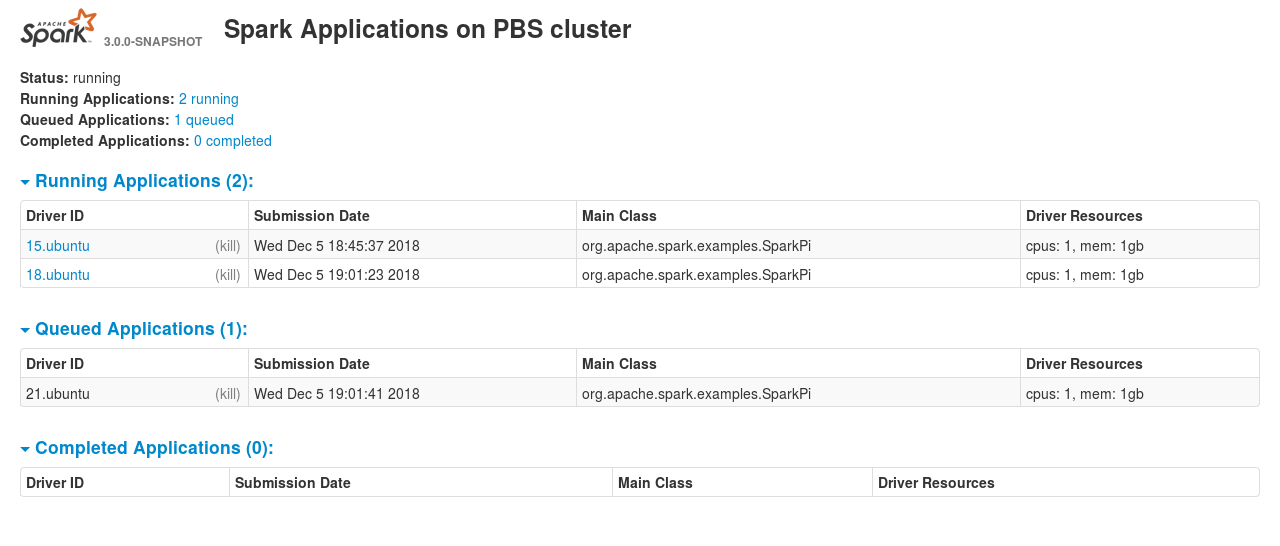
\includegraphics[width=0.75 \textwidth, natwidth=1280, natheight=900]
            {assets/images/Cluster.png}
        }
    \caption{Spark Cluster UI page displaying jobs on PBS Cluster}
\end{figure}

\subsection{Job submission in PBS}
\paragraph{}
The job submission in \glssymbol{pbs} is done via \texttt{qsub} command. The
parameters of a typical job submission include the number of CPU cores, the
amount of memory and the \gls{walltime} for the job.

\subsection{Overriding Spark's cluster manager}
\paragraph{}
There is already support in \gls{spark} codebase for \gls{yarn}, \gls{mesos} and
\gls{kubernetes}. This is done by overriding the \texttt{ExternalClusterManager}
in Spark. This class is responsible to create an instance of
\texttt{SchedulerBackend} which we also override. The \texttt{SchedulerBackend}
is responsible to start the \glspl{executor} and we change that so that it
now submits the \glspl{executor} as jobs to \glssymbol{pbs} instead.

\begin{figure}[h]
    \centering
    \fbox{
        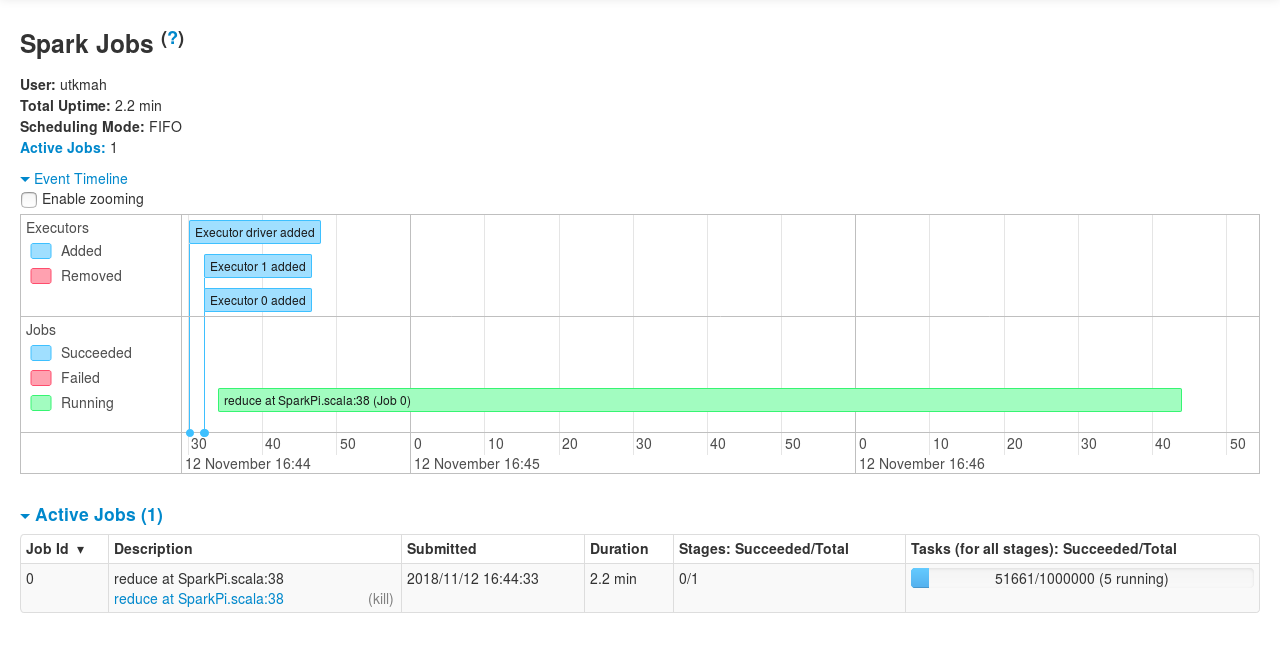
\includegraphics[width=0.75 \textwidth, natwidth=1280, natheight=849]
            {assets/images/Jobs.png}
        }
    \caption{Spark Job page for each Spark Driver}
\end{figure}

\paragraph{}
The above setup works well for a job where the \gls{driver} is run locally. But
to allow the \gls{driver} to run remotely on a cluster, we must also be able to
submit the \gls{driver} as a \glssymbol{pbs} job. To do this, we also override
\texttt{SparkApplication} which is instantiated whenever a \gls{spark} job is
submitted. This is responsible to start the \gls{driver} which we now just start
as a \glssymbol{pbs} job.

\begin{figure}[h]
    \centering
    \fbox{
        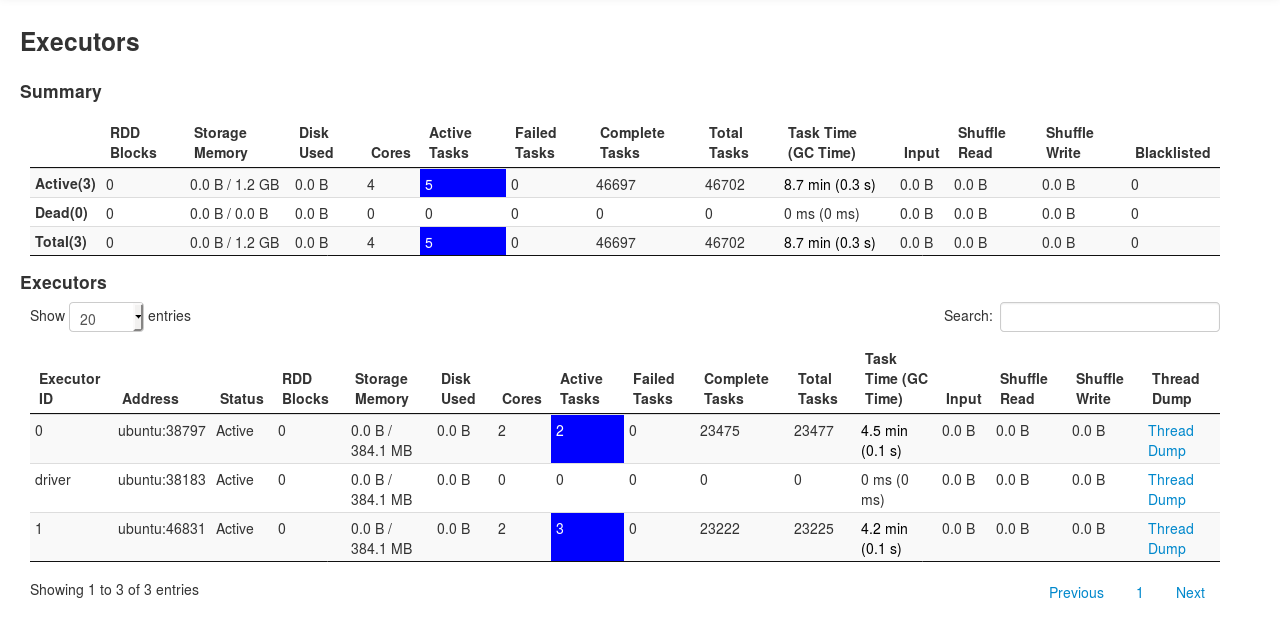
\includegraphics[width=0.75 \textwidth, natwidth=1280, natheight=849]
            {assets/images/Executors.png}
        }
    \caption{Job page listing executors which are running on PBS cluster nodes}
\end{figure}


\section{Result}

\subsection{Installation}
\paragraph{}
The \gls{spark} application has to be patched to allow setting \glssymbol{pbs}
as a scheduler. Apart from this, the \gls{spark} application must be compiled
with the overridden classes. This whole compiled version of \gls{spark} must be
installed on each execution node of the cluster as well as the client node.

\subsection{Usage}
\paragraph{}
The \gls{spark} application can be submitted just like it used to be submitted
before the \glssymbol{pbs} integration with the commands following the similar
pattern:
\begin{lstlisting}
    bin/spark-shell --master pbs

    bin/spark-submit --master pbs --deploy-mode client \
        --class <main-class> <application-jar> [application args]

    bin/spark-submit --master pbs --deploy-mode cluster \
        --class <main-class> <application-jar> [application args]
\end{lstlisting}

\begin{figure}[h]
    \centering
    \fbox{
        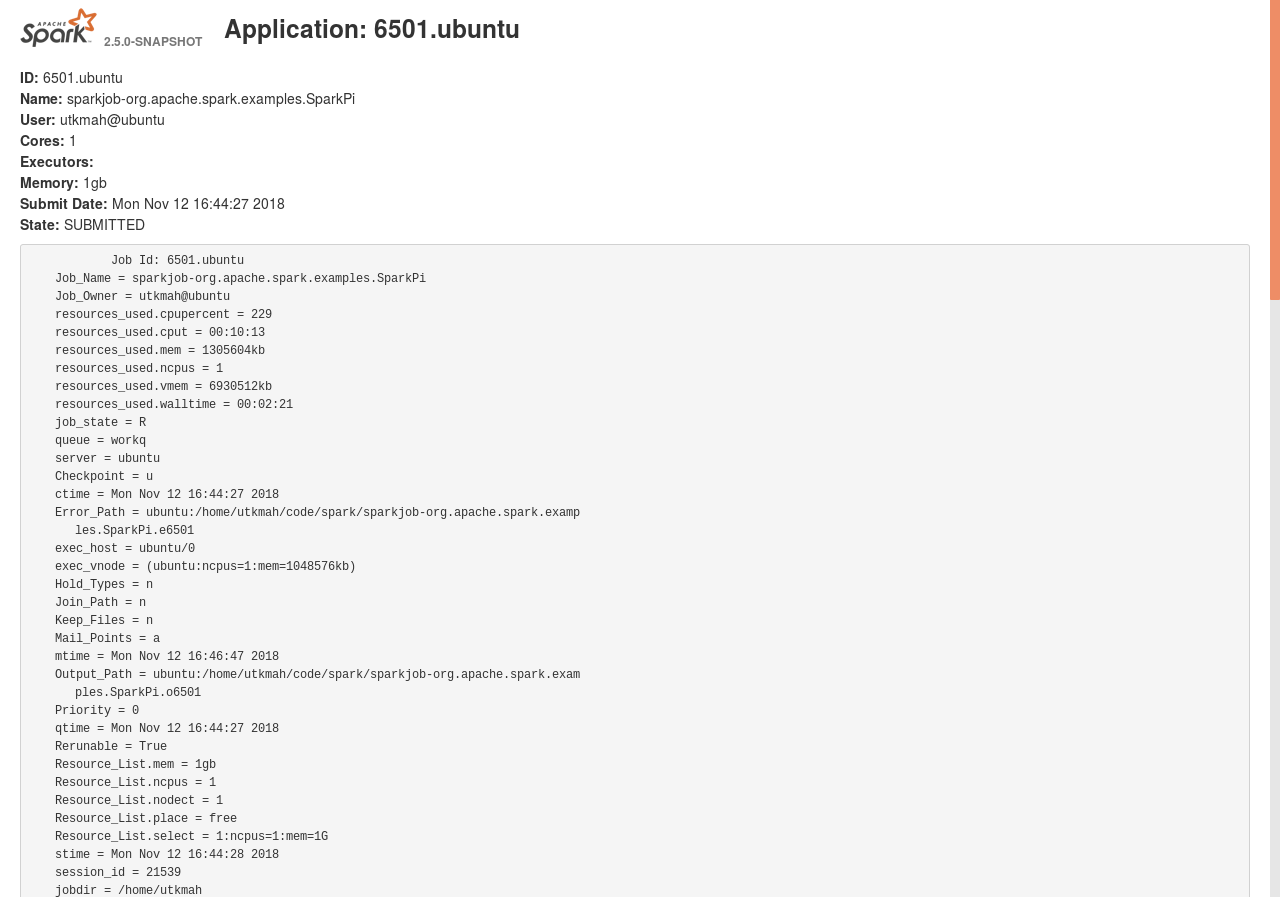
\includegraphics[width=0.75 \textwidth, natwidth=1280, natheight=897]
            {assets/images/App.png}
        }
    \caption{Spark Application page displaying PBS Job properties}
\end{figure}
